\chapter{Les transistors}
\section{Le transistor : généralités}
Il s'agit d'un élément pouvant être utilisé en \textit{amplification} (électronique 
analogique, AOP, \dots) ou en \textit{commutation} (base de l'électronique numérique). 
On les regroupe en deux familles : les transistors \textit{bipolaires} et à 
\textit{effet de champ}. Cette dernière famille est la plus utilisée aujourd'hui : 
dans ce chapitre, nous étudierons le NMOS à enrichissement, transistor à effet de champ.

\section{Le transistor MOS utilisé en amplification}
	\subsection{Transistor MOS : propriétés de base}
		\subsubsection{Introduction}
				\begin{wrapfigure}[6]{r}{2cm}
		\vspace{-1cm}
		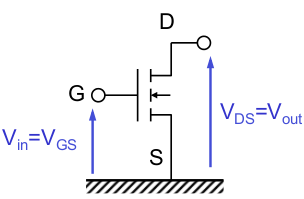
\includegraphics[scale=0.35]{ch7/image1}
		\captionof{figure}{ }
		\end{wrapfigure}
	Le transistor possède trois bornes ; les trois bornes du NMOS se nomment le 
	\textit{drain} (D), la \textit{source} (S) et la grille (G). Qui dit trois bornes 
	dit plusieurs modes de connexion : souvent la source est utilisée comme référence 
	de tension par rapport à la grille et au drain, c'est une \textbf{source commune}, 
	source que l'on connecte à la masse.\\

		\begin{wrapfigure}[5]{l}{4.5cm}
	\vspace{-0.5cm}
	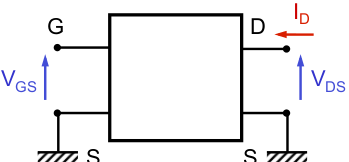
\includegraphics[scale=0.35]{ch7/image2}
		\captionof{figure}{ }
		\end{wrapfigure}	
	Dans un tel montage, on applique au transistor la tension $V_{GS}$ (signal d'entrée) 
	et en récupère la tension $V_{DS}$ (signal de sortie). Sous cette disposition, on 
	peut associer le transistor à un quadripôle (ou la source est commune à l'entrée et 
	à la sortie, étant reliée à la masse).\footnote{On considère un courant (entrant par 
	convention) à la sortie et aucun courant à l'entrée (cf. plus tard)}
	
	
	\subsubsection{Caractéristique de sortie}
			\begin{wrapfigure}[7]{r}{6cm}
	\vspace{-0.8cm}
	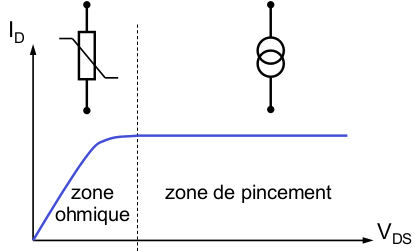
\includegraphics[scale=0.4]{ch7/image3}
		\captionof{figure}{ }
		\end{wrapfigure}	
	On s'intéresse ici à la courbe décrivant le comportement du transistor dans le plan 
	$(I_D,V_{DS})$. Soit $I_D$ le courant de drain, c'est-à-dire le courant traversant 
	le transistor du drain vers la source. Au début, lorsque les signaux sont faibles, 
	la caractéristique comporte une zone dite \textit{zone ohmique} : on associe le 
	comportement à celui d'une résistance (droite) non-linéaire (s'incurve).
	
\newpage	
			\begin{wrapfigure}[8]{r}{6cm}
	\vspace{-0.5cm}
	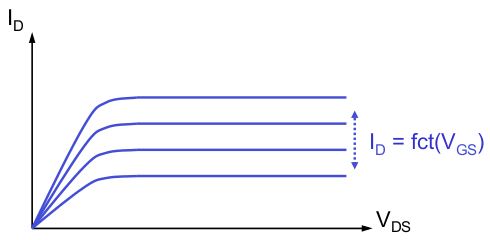
\includegraphics[scale=0.4]{ch7/image4}
		\captionof{figure}{ }
		\end{wrapfigure}	
	 Pour de 
	plus grandes valeurs de $V_{DS}$, la caractéristique est horizontale : on associe 
	le comportement de cette zone, dite \textit{zone de pincement} à celui d'une 
	source de courant. Le transistor fonctionne alors comme une \textbf{source de courant} 
	si la tension $V_{DS}$ qu'on lui applique est suffisante.\\
	
	Il ne faut pas oublier que la valeur du courant de drain $I_D$ dépend de $V_{GS}$ appliquée 
	au transistor (dépendance non-linéaire) : 
	la caractéristique de 
	sortie est un réseau de courbe dont une seule n'est vrai qu'à un instant donné! Si 
	on demande la caractéristique d'un MOS à l'examen, il faut bien donner le réseau de 
	courbes\footnote{\danger Ne pas confondre $V_{DS}$ et $V_{GS}$ !}.
	
	\subsubsection{Caractéristique de transfert}
	\begin{wrapfigure}[8]{r}{4.5cm}
	\vspace{-0.8cm}
	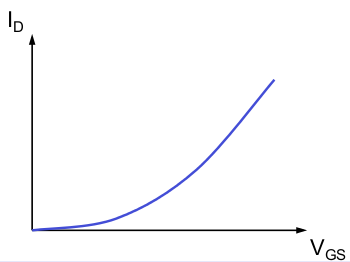
\includegraphics[scale=0.4]{ch7/image5}
	\captionof{figure}{ }
	\end{wrapfigure}	
	Cette caractéristique représente la dépendance entre $I_D$ et $V_GS$. On place 
	la grandeur de sortie en ordonnée ($I_D$ et la grandeur d'entrée en abscisse 
	($V_{GS}$). La relation est non-linéaire, représenté ci-contre uniquement avec 
	pincement (la représentation est d'ailleurs un peu faussée, il faudrait légèrement 
	translater la courbe vers la droite).
	
	\subsubsection{Caractéristique de transfert : transconductance}	
	On appelle la pente de la caractéristique de transfert est la transconductance :
	\begin{equation}
	g_m = \left.\dfrac{\delta I_D}{\delta V_{GS}}\right|_Q
	\end{equation}
	Elle varie en fonction du point $Q$ considéré et son unité s'exprime en 
	$\Omega^{-1}$. Il s'agit du facteur multiplicatif entre l'entée et la sortie que 
	l'on ne peut appeler gain car l'entrée et la sortie ne sont pas du même type (tension 
	et courant).
	
	
	
	\subsection{Transistor MOS : structure interne}	
	Voir chapitre 6.
	
	\subsection{Étage amplificateur à transistor MOS : principe}
		\subsubsection{Étage amplificateur}
			\begin{wrapfigure}[11]{l}{3.5cm}
	\vspace{-0.5cm}
	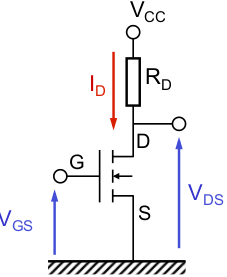
\includegraphics[scale=0.4]{ch7/image6}
	\captionof{figure}{ }
	\end{wrapfigure}
		On vient de voir que le transistor agit comme une source de \textbf{courant} 
		commandée en \textbf{tension}. Pour faire une source de \textbf{tension} 
		commandée en \textbf{tension} il suffit de rajouter une résistance ! On peut 
		alors parler de gain. Ci-contre, l'\textbf{étage amplificateur à source 
		commune} : schéma de base pour l'amplification. \\
		
		On peut voir $V_{CC}$ comme une source externe d'énergie utilisable par le 
		transistor, celui-ci va la "doser" : le transistor est un élément actif qui 
		contrôle un signal d'énergie élever par un signal plus faible. On suppose 
		ici un montage à vide, sans charge : le courant dans la résistance est le 
		même que celui traversant le transistor entre D et S ($I_D$).
	
	
		\subsubsection{Étage amplificateur : résolution graphique}
					\begin{wrapfigure}[11]{r}{5.5cm}
	\vspace{-0.5cm}
	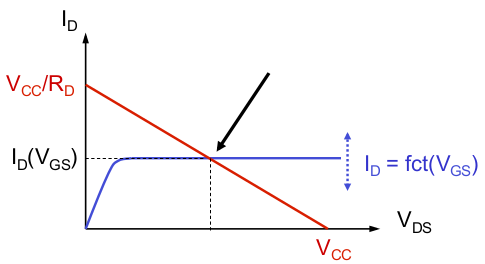
\includegraphics[scale=0.4]{ch7/image7}
	\captionof{figure}{ }
	\end{wrapfigure}
		La question est : que vaut $V_{DS}$ ? La résolution graphique est préférable, 
		l'analytique étant lourde à cause de la non-linéarité du composant : on va 
		tout tracer dans le même graphique. La résistance impose 
		\begin{equation}
		V = R_D.I_D
		\end{equation}
		On peut donc écrire la chute de tension sur $R_D$ :
		\begin{equation}
		V_{DS} = V_CC - R_D.I_D
		\end{equation}
		On peut alors obtenir une droite nommée \textit{droite de charge}. 
		L'intersection de cette droite avec la caractéristique de sortie nous donne 
		le point de fonctionnement \textbf{à un moment donné}. Cependant, n'oublions 
		pas que nous avons un "réseau" de courbes : l'intersection n'est pas fixe, 
		elle dépend de la tension d'entrée du montage (soit la valeur de la tension 
		de grille $V_{GS}$).
	
	\subsubsection{Étage amplificateur: interprétation}
	Lorsqu'on augmente $V_{GS}$ le transistor consomme de plus en plus de courant
	$I_D$ : la caractéristique de sortie se translate vers le haut. Forcément, la 
	chute de tension sur $R_D$ augmente et $V_{DS}$ diminue (à cause d'une chute 
	plus importante dans la résistance).
	
	\subsubsection{Étage amplificateur: difficultés}
	Peut-on parler d'amplification ($V_{GS}$ par rapport à $V_{DS}$) ? Ahah, non. Trois 
	raisons :
	\begin{enumerate}
	\item Le gain en tension est négatif (on vient de voir qu'augmenter $V_{GS}$ diminue 
	$V_{DS}$
	\item L'amplification est non linéaire (caractéristique de transfert du transistor)
	\item Pas d'amplification si $V_{GS} < 0$ (structure interne)
	\end{enumerate}
	
	\subsubsection{Polarisation}
	\begin{wrapfigure}[8]{r}{9.5cm}
	\vspace{-0.5cm}
	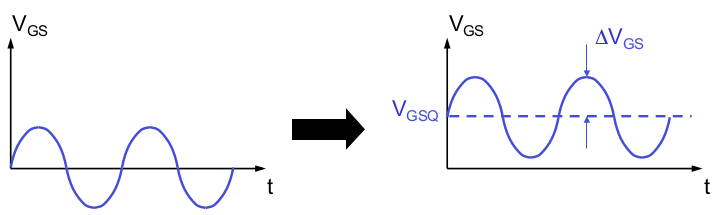
\includegraphics[scale=0.4]{ch7/image8}
	\captionof{figure}{ }
	\end{wrapfigure}
	Le troisième problème est gênant, car énormément de signaux sont alternatifs : il 
	faut décaler $V_{GS}$ pour que toutes ses valeurs soient positives en lui rajoutant 
	une composante continue. Le signal d'entrée possède alors une composante $V_{GSQ}$ 
	soit une tension continue (moyenne du signal $V_{GS}$) et une composante alternative 
	portant l'information utile $\Delta V_{GS}$. La présence de ce terme continue s'étend 
	alors aux autres grandeurs électriques : $I_D = I_{DQ} + \Delta I_D$ et $V_{DS} = 
	V_{DSQ}+\Delta V_{DS}$. Cette composante continue est la \textbf{polarisation} : elle 
	ne porte aucune information utile et sert juste à placer le transistor dans une 
	certaine condition électrique\footnote{Le point de polarisation est le point correspondant 
	aux valeurs moyennes des signaux électriques.}
	
	\subsubsection{Petites signaux}
	L'amplification étant non-linéaire\footnote{La caractéristique de transfert est non 
	linéaire.}, l'amplification l'est donc également : distorsions. Pour régler ce problème, 
	on linéarise le système avec l'utilisation de faibles signaux 	afin d'assimiler la courbe 
	à sa tangente. Pour le problème du gain négatif, ça n'en est pas vraiment un. Au pire, 
	il faut juste rajouter un second étage pour ré-inverser le tout.

	\subsubsection{Étage amplificateur : interprétation}
	\begin{center}
	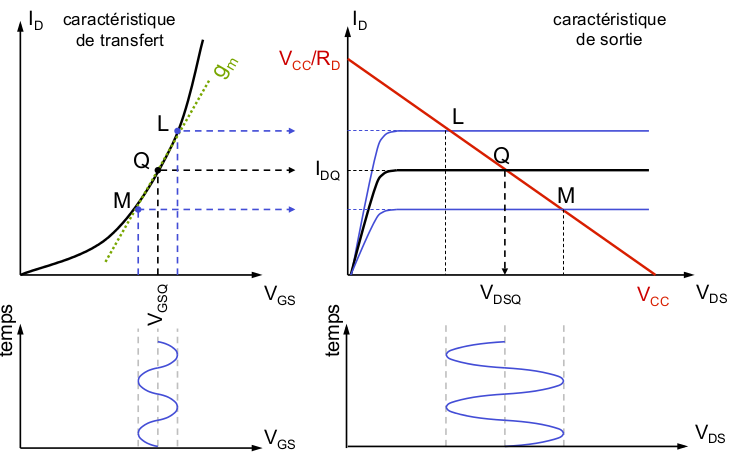
\includegraphics[scale=0.5]{ch7/image9}
	\captionof{figure}{ }
	\end{center}
	Considérons que notre fonction d'entrée (bas-gauche) soit un sinus placé au milieu de 
	son axe par une polarisation d'entrée. Nous pouvons reporter l'amplitude d'oscillation 
	sur le graphique du dessus (haut-gauche), les abscisses correspondant. Même si les 
	oscillations sont petites, la droite est très forte est les variations seront importantes. 
	En reportant $I_D$ (haut-droite) et en suivant un raisonnement similaire on retrouve la 
	tension de sortie (composante alternative), amplifiée négativement.
	
	
	
	
	\subsection{Étage amplificateur à transistor MOS: calcul}
		\subsubsection{Introduction}
		Il faut séparer la polarisation et les petits signaux (composante alternative à 
		amplifier) :
		\begin{itemize}
		\item[$\bullet$] Polarisation ; grandeurs continues (DC)
		\item[$\bullet$] Petits signaux ; grandeurs alternatives (AC)		
		\end{itemize}
	
		Que vaut dès lors notre gain ? Les calculs sont assez simples et repris dans les 
		slides 43-45 (\danger examen).
		\begin{equation}
		A_{AC} = \dfrac{\delta V_{DS}}{\delta V_{GS}} = -g_mR_D
		\end{equation}
		
	
	
	
	
	
	
	
	
	
	
	
	
	
	
	
	
	
	
	
	
	
	